\sectionthree{Multi-tape TM}
\begin{python0}
from solutions import *; clear()
\end{python0}

Consider a version of the TM where there are multiple tapes. The
input is placed on the first. The TM has one read/write head for
each tape.
(The read/write head for each tape can even have
the ability to read/write a different set of characters.)
Say this TM has $k$ read/write heads (and $k$ tapes).
Then the transition function is of the form
\[
\delta : Q \times \Gamma^k \rightarrow Q \times \Gamma^k \times \{L,R,S\}^k
\]
The input for such a $k$--tape machine is placed on the first tape.


For instance suppose there's a 2-tape TM that is currently
at state $q$ and the two input tapes look like this:
\begin{center}
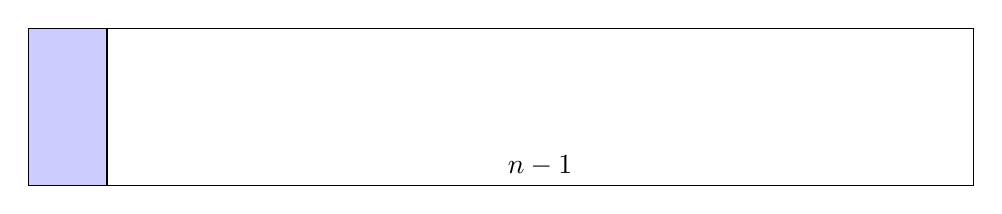
\begin{tikzpicture}

\draw (6.0, 1.0)
  node[draw, , , color=black,
       rounded corners=0cm, inner sep=0cm] {

\begin{minipage}[t][2cm]{12cm}
\mbox{}

\end{minipage}

};
\draw (0.5, 1.0)
  node[fill=blue!20!white,rounded corners=0cm,inner sep=0cm] {

\begin{minipage}[t][2cm]{1cm}
\mbox{}

\end{minipage}

};
\draw (0.5, 1.0)
  node[draw, , , color=black,
       rounded corners=0cm, inner sep=0cm] {

\begin{minipage}[t][2cm]{1cm}
\mbox{}

\end{minipage}

};
\draw (6.5, 0.25)
  node[draw=none, line width=0cm, , color=black,
       rounded corners=0cm, inner sep=0cm] {

\begin{minipage}[t][0.1cm]{0.1cm}
\mbox{}

\end{minipage}

};\draw (6.5, 0.25) node[color=black] {$n - 1$};
\end{tikzpicture}

\end{center}


(For readability, I've assumed the TM mark the end-of-tape for each tape.)

Note that there are two read/write heads (look at the arrows
above), the first read/write
head is about to read the fourth character on the first tape
and the second is about to read the sixth character on the second
tape.
Suppose the
relevant transition is
\[
\delta(q, (a, \sqcup)) = (q', (b, a), (L, R))
\]
i.e., this is part of the TM diagram:
\begin{center}
\begin{tikzpicture}[shorten >=1pt,node distance=2cm,auto,initial text=]
\node[state] (q) at (0,0) {$q$};
\node[state] (q1) at (6,0) {$q'$};

\path[->]
(q) edge [above] node {$(a,\sqcup) \rightarrow (b,a), (L,R)$} (q1)
;
\end{tikzpicture}
\end{center}
On running the transition the TM is at state $q'$ and the
tapes look like:
\begin{center}
\begin{tikzpicture}

\fill[blue!10] (0.0, 0.0) circle (0.3);
\node [line width=0.03cm,black,minimum size=0.57cm,draw,circle] at (0.0,0.0)(a){};\draw (0.0, 0.0) node[color=black] {$a$};
\fill[blue!10] (-2.0, -1.0) circle (0.3);
\node [line width=0.03cm,black,minimum size=0.57cm,draw,circle] at (-2.0,-1.0)(b){};\draw (-2.0, -1.0) node[color=black] {$b$};
\fill[blue!10] (2.0, -1.0) circle (0.3);
\node [line width=0.03cm,black,minimum size=0.57cm,draw,circle] at (2.0,-1.0)(d){};\draw (2.0, -1.0) node[color=black] {$d$};
\fill[blue!10] (-3.0, -2.0) circle (0.3);
\node [line width=0.03cm,black,minimum size=0.57cm,draw,circle] at (-3.0,-2.0)(e){};\draw (-3.0, -2.0) node[color=black] {$e$};
\fill[blue!10] (-1.0, -2.0) circle (0.3);
\node [line width=0.03cm,black,minimum size=0.57cm,draw,circle] at (-1.0,-2.0)(f){};\draw (-1.0, -2.0) node[color=black] {$f$};
\fill[blue!10] (1.0, -2.0) circle (0.3);
\node [line width=0.03cm,black,minimum size=0.57cm,draw,circle] at (1.0,-2.0)(h){};\draw (1.0, -2.0) node[color=black] {$h$};
\fill[blue!10] (3.0, -2.0) circle (0.3);
\node [line width=0.03cm,black,minimum size=0.57cm,draw,circle] at (3.0,-2.0)(o){};\draw (3.0, -2.0) node[color=black] {$o$};
\fill[blue!10] (-2.5, -3.0) circle (0.3);
\node [line width=0.03cm,black,minimum size=0.57cm,draw,circle] at (-2.5,-3.0)(l){};\draw (-2.5, -3.0) node[color=black] {$l$};
\fill[blue!10] (1.5, -3.0) circle (0.3);
\node [line width=0.03cm,black,minimum size=0.57cm,draw,circle] at (1.5,-3.0)(m){};\draw (1.5, -3.0) node[color=black] {$m$};
\fill[blue!10] (3.5, -3.0) circle (0.3);
\node [line width=0.03cm,black,minimum size=0.57cm,draw,circle] at (3.5,-3.0)(j){};\draw (3.5, -3.0) node[color=black] {$j$};\draw[line width=0.03cm,black,->,>=triangle 60] (a) to  (b);
\draw[line width=0.03cm,black,->,>=triangle 60] (a) to  (d);
\draw[line width=0.03cm,black,->,>=triangle 60] (b) to  (e);
\draw[line width=0.03cm,black,->,>=triangle 60] (b) to  (f);
\draw[line width=0.03cm,black,->,>=triangle 60] (d) to  (h);
\draw[line width=0.03cm,black,->,>=triangle 60] (d) to  (o);
\draw[line width=0.03cm,black,->,>=triangle 60] (e) to  (l);
\draw[line width=0.03cm,black,->,>=triangle 60] (h) to  (m);
\draw[line width=0.03cm,black,->,>=triangle 60] (o) to  (j);
\end{tikzpicture}

\end{center}



Is this machine more powerful? No. You can prove that
it's as powerful as the ``regular'' TM. In other words given a
$k$--tape TM $M$, there is a $1$--tape TM $M'$ such that $L(M) =
L(M')$.

As an example, if a 2-tape TM has this tape configuration:
\begin{center}
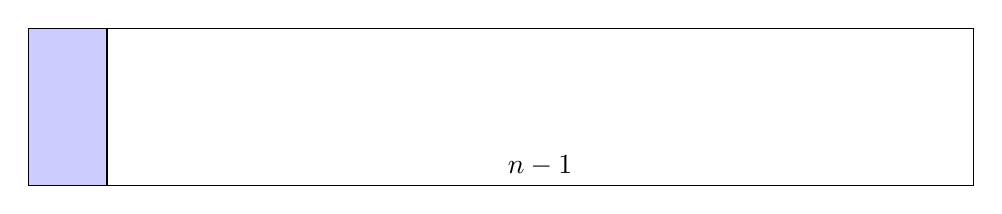
\begin{tikzpicture}

\draw (6.0, 1.0)
  node[draw, , , color=black,
       rounded corners=0cm, inner sep=0cm] {

\begin{minipage}[t][2cm]{12cm}
\mbox{}

\end{minipage}

};
\draw (0.5, 1.0)
  node[fill=blue!20!white,rounded corners=0cm,inner sep=0cm] {

\begin{minipage}[t][2cm]{1cm}
\mbox{}

\end{minipage}

};
\draw (0.5, 1.0)
  node[draw, , , color=black,
       rounded corners=0cm, inner sep=0cm] {

\begin{minipage}[t][2cm]{1cm}
\mbox{}

\end{minipage}

};
\draw (6.5, 0.25)
  node[draw=none, line width=0cm, , color=black,
       rounded corners=0cm, inner sep=0cm] {

\begin{minipage}[t][0.1cm]{0.1cm}
\mbox{}

\end{minipage}

};\draw (6.5, 0.25) node[color=black] {$n - 1$};
\end{tikzpicture}

\end{center}


the 1-tape regular TM can simulate the above with this tape:
\begin{center}
\begin{tikzpicture}

\fill[blue!10] (0.0, 0.0) circle (0.3);
\node [line width=0.03cm,black,minimum size=0.57cm,draw,circle] at (0.0,0.0)(a){};\draw (0.0, 0.0) node[color=black] {$a$};
\fill[blue!10] (-2.0, -1.0) circle (0.3);
\node [line width=0.03cm,black,minimum size=0.57cm,draw,circle] at (-2.0,-1.0)(b){};\draw (-2.0, -1.0) node[color=black] {$b$};
\fill[blue!10] (2.0, -1.0) circle (0.3);
\node [line width=0.03cm,black,minimum size=0.57cm,draw,circle] at (2.0,-1.0)(d){};\draw (2.0, -1.0) node[color=black] {$d$};
\fill[blue!10] (-3.0, -2.0) circle (0.3);
\node [line width=0.03cm,black,minimum size=0.57cm,draw,circle] at (-3.0,-2.0)(e){};\draw (-3.0, -2.0) node[color=black] {$e$};
\fill[blue!10] (-1.0, -2.0) circle (0.3);
\node [line width=0.03cm,black,minimum size=0.57cm,draw,circle] at (-1.0,-2.0)(f){};\draw (-1.0, -2.0) node[color=black] {$f$};
\fill[blue!10] (1.0, -2.0) circle (0.3);
\node [line width=0.03cm,black,minimum size=0.57cm,draw,circle] at (1.0,-2.0)(m){};\draw (1.0, -2.0) node[color=black] {$m$};
\fill[blue!10] (3.0, -2.0) circle (0.3);
\node [line width=0.03cm,black,minimum size=0.57cm,draw,circle] at (3.0,-2.0)(o){};\draw (3.0, -2.0) node[color=black] {$o$};
\fill[blue!10] (-3.5, -3.0) circle (0.3);
\node [line width=0.03cm,black,minimum size=0.57cm,draw,circle] at (-3.5,-3.0)(k){};\draw (-3.5, -3.0) node[color=black] {$k$};
\fill[blue!10] (-2.5, -3.0) circle (0.3);
\node [line width=0.03cm,black,minimum size=0.57cm,draw,circle] at (-2.5,-3.0)(l){};\draw (-2.5, -3.0) node[color=black] {$l$};
\fill[blue!10] (3.5, -3.0) circle (0.3);
\node [line width=0.03cm,black,minimum size=0.57cm,draw,circle] at (3.5,-3.0)(j){};\draw (3.5, -3.0) node[color=black] {$j$};\draw[line width=0.03cm,black,->,>=triangle 60] (a) to  (b);
\draw[line width=0.03cm,black,->,>=triangle 60] (a) to  (d);
\draw[line width=0.03cm,black,->,>=triangle 60] (b) to  (e);
\draw[line width=0.03cm,black,->,>=triangle 60] (b) to  (f);
\draw[line width=0.03cm,black,->,>=triangle 60] (d) to  (m);
\draw[line width=0.03cm,black,->,>=triangle 60] (d) to  (o);
\draw[line width=0.03cm,black,->,>=triangle 60] (e) to  (k);
\draw[line width=0.03cm,black,->,>=triangle 60] (e) to  (l);
\draw[line width=0.03cm,black,->,>=triangle 60] (o) to  (j);
\end{tikzpicture}

\end{center}


Note that the asterisk in \texttt{a$^*$} in the regular TM
records the fact the for the corresponding 2-tape TM,
the first read/write head is about to read this \texttt{a}.
Nice idea right?
In general for each character in the $\Gamma$ of the 2-tape machine,
there are two characters in the $\Gamma$ of the 1-tape machine.
So for the above example the 2-tape TM has
$\Gamma = \{\texttt{a}, \texttt{b}, \sqcup\}$
and the $\Gamma$ of the corresponding 1-tape TM is
$\{\texttt{a}, \texttt{a$^*$},
\texttt{b}, \texttt{b$^*$},
\sqcup, \sqcup^*, \texttt{\$}\}$

Here's how this TM $M'$ works.
If initially the input is say $aaba$ for the 2-tape $M$ (on the first tape),
$M'$ will initialize the tape this way:
\begin{center}
\begin{tikzpicture}

\fill[blue!10] (0.0, 0.0) circle (0.3);
\node [line width=0.03cm,black,minimum size=0.57cm,draw,circle] at (0.0,0.0)(a){};\draw (0.0, 0.0) node[color=black] {$a$};
\fill[blue!10] (-2.0, -1.0) circle (0.3);
\node [line width=0.03cm,black,minimum size=0.57cm,draw,circle] at (-2.0,-1.0)(b){};\draw (-2.0, -1.0) node[color=black] {$b$};
\fill[blue!10] (2.0, -1.0) circle (0.3);
\node [line width=0.03cm,black,minimum size=0.57cm,draw,circle] at (2.0,-1.0)(d){};\draw (2.0, -1.0) node[color=black] {$d$};
\fill[blue!10] (-3.0, -2.0) circle (0.3);
\node [line width=0.03cm,black,minimum size=0.57cm,draw,circle] at (-3.0,-2.0)(e){};\draw (-3.0, -2.0) node[color=black] {$e$};
\fill[blue!10] (-1.0, -2.0) circle (0.3);
\node [line width=0.03cm,black,minimum size=0.57cm,draw,circle] at (-1.0,-2.0)(f){};\draw (-1.0, -2.0) node[color=black] {$f$};
\fill[blue!10] (1.0, -2.0) circle (0.3);
\node [line width=0.03cm,black,minimum size=0.57cm,draw,circle] at (1.0,-2.0)(m){};\draw (1.0, -2.0) node[color=black] {$m$};
\fill[blue!10] (3.0, -2.0) circle (0.3);
\node [line width=0.03cm,black,minimum size=0.57cm,draw,circle] at (3.0,-2.0)(j){};\draw (3.0, -2.0) node[color=black] {$j$};
\fill[blue!10] (-3.5, -3.0) circle (0.3);
\node [line width=0.03cm,black,minimum size=0.57cm,draw,circle] at (-3.5,-3.0)(k){};\draw (-3.5, -3.0) node[color=black] {$k$};
\fill[blue!10] (-2.5, -3.0) circle (0.3);
\node [line width=0.03cm,black,minimum size=0.57cm,draw,circle] at (-2.5,-3.0)(l){};\draw (-2.5, -3.0) node[color=black] {$l$};\draw[line width=0.03cm,black,->,>=triangle 60] (a) to  (b);
\draw[line width=0.03cm,black,->,>=triangle 60] (a) to  (d);
\draw[line width=0.03cm,black,->,>=triangle 60] (b) to  (e);
\draw[line width=0.03cm,black,->,>=triangle 60] (b) to  (f);
\draw[line width=0.03cm,black,->,>=triangle 60] (d) to  (m);
\draw[line width=0.03cm,black,->,>=triangle 60] (d) to  (j);
\draw[line width=0.03cm,black,->,>=triangle 60] (e) to  (k);
\draw[line width=0.03cm,black,->,>=triangle 60] (e) to  (l);
\end{tikzpicture}

\end{center}



Suppose $M$ is at state $q$.
$M'$ will then scan left to locate the marked characters
Once it reaches the second \texttt{!}, it knows that the
two characters that the corresponding 2-tape machine is looking
at. Say it's $(c,c')$.
Then $M'$ \lq\lq remember'' that it should be at
state $q$ and should be reading character $(c,c')$.
In other words $M'$ enters state $(q,c,c')$ -- the new TM $M'$ that
simulates $M$ must have such states.
The TM $M'$ now \lq\lq knows'' the current state of computation of $M$.

Based on how the original $M$ works, i.e., based on the transition
of $M$ at state $q$ and reading $(c,c')$, the corresponding
machine $M'$ now scans left and simulate what $M$ should do,
modify the input tape as it scans.

I'll leave the rest to you -- there are lots of details to work out,
but it's not difficult once you get the idea of merging multiple
tape segments onto one long tape.
